% testProcedure.tex
\subsection{Source Code Repository}
PR37 MS7 arm uses a different architecture than MS5/6 arm. The branch of each repository is listed below:
\begin{itemize}
	\item keos: release/1.9
	\item bitwin: release/1.1
	\item rtcontrol\_nextgen: release/1.1
	\item sdk\_assitive: temp\_logButton* 
\end{itemize}

temp\_logButton is modified from release/1.1, with only one modification on the data log buttons. In this branch, "START LOG" and "STOP LOG" buttons will activate/deactivate the rtcontrol logger, instead of NOVA logger. This modification is a temporal change for this test only. Because at the moment of test, rtcontrol cannot log data when robot was in a static position.

\subsection{Data acquisition}
Make sure change the joint positions in "traj/mainTrajectories.csv" in NOVA installation folder to the predefined configurations shown in Section \ref{sec:testSetup}.
\begin{enumerate}
	\item run executable rtcontrol on QNX
	\item run sdk\_assitive to get NOVA interface on PC (as in Figure \ref{fig:nova})
	\item select AURIS in NOVA
	\item select AURIS Control in NOVA
	\item set IP of QNX, Run Mode in "run", and then click Connect
	\item release robot break
	\item select a pose in the list of "Configuration Selection" and press "SEND SELECTED" button
	\item when robot motion finished, click "START LOG", and then click "STOP LOG" aproximately 2 seconds later
	\item copy and rename the log file according to the index of pre-defined configuration
	\item input a new pre-defined robot configuration and repeat the steps to get data log for all pre-defined robot configurations
\end{enumerate}

\begin{figure}
	\begin{center}
		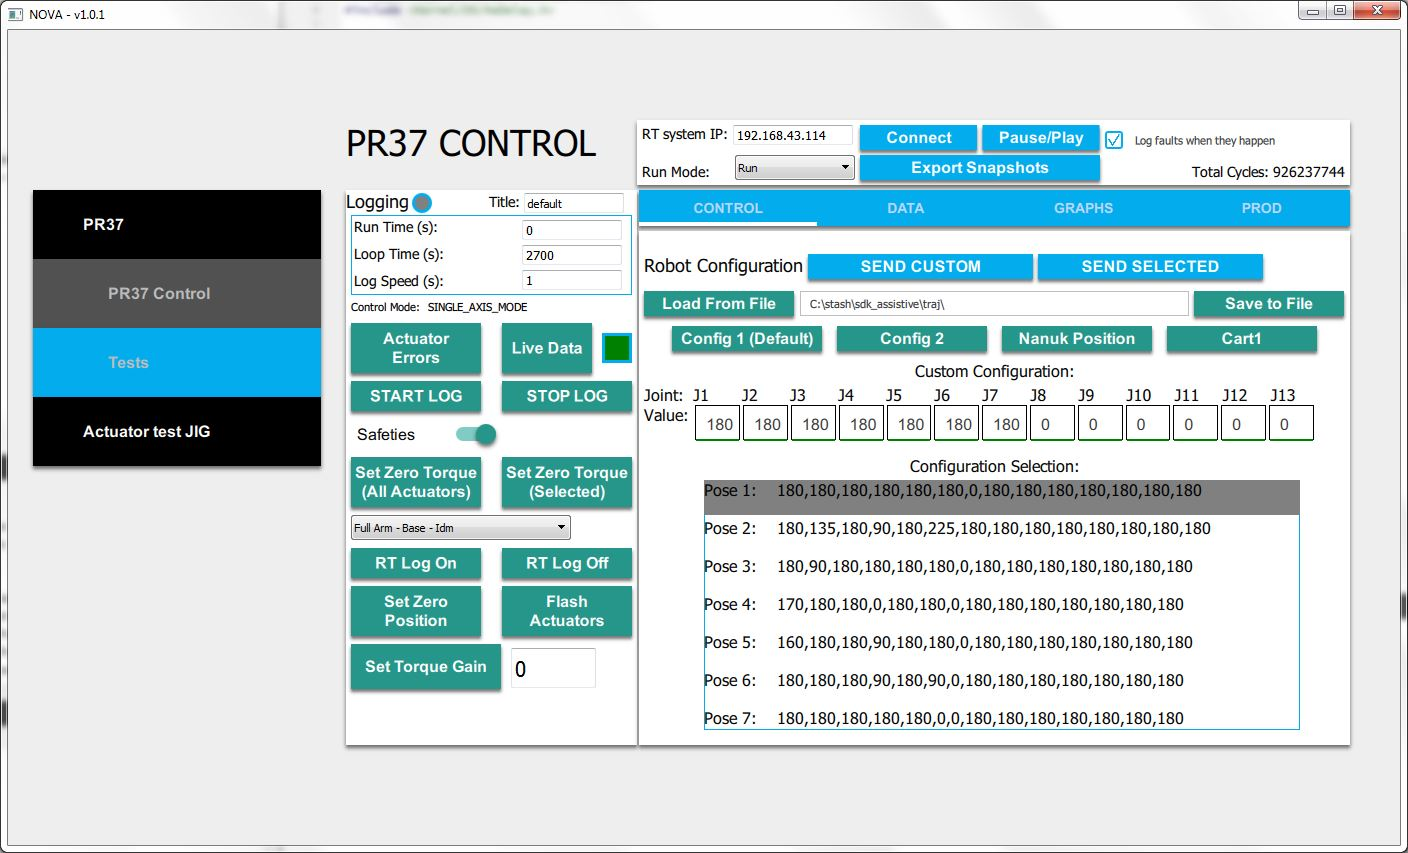
\includegraphics[width=0.9\textwidth]{./images/NOVA.JPG}%
		\caption{NOVA interface}
		\label{fig:nova}%
	\end{center}
\end{figure}
